\documentclass[11pt,a4paper]{article}


\setlength{\topmargin}{-55pt}%
\setlength{\oddsidemargin}{-20pt}%
\setlength{\textwidth}{490pt}%
\setlength{\textheight}{700pt}%
\setlength{\headsep}{20pt}%
\setlength{\headheight}{14pt}

\usepackage[utf8]{inputenc} % accents 8 bits dans le fichier
\usepackage[T1]{fontenc}      % accents codés dans la fonte
\usepackage[french]{babel}
\usepackage{amsmath,amssymb}
\usepackage{graphicx}
\usepackage{fancyhdr}
\usepackage{booktabs}
\usepackage{color, colortbl}
\usepackage{appendix}
\usepackage{pgfplots}
\usepackage[hidelinks]{hyperref}
\usepackage{siunitx}
\usepackage{algorithmicx}
\usepackage{algorithm}
\usepackage{algpseudocode}

\pgfplotsset{compat=1.3}

\addto\captionsfrench{% Replace "english" with the language you use
  \renewcommand{\contentsname}%
    {Table des matières}
}

\DecimalMathComma

\lhead{}      %en-tête
\chead{MPNA : Méthode des itérations simultanées}%
\rhead{}%
\lfoot{\tiny{Pierre GRANGER \& Matthias BEAUPERE}}
\cfoot{}%
\rfoot{\thepage}%
\renewcommand{\headrulewidth}{0.5pt}
\renewcommand{\footrulewidth}{0.5pt}
\pagestyle{fancy}

\newcommand{\HRule}{\rule{\linewidth}{0.5mm}}

\definecolor{green}{rgb}{0.2,0.8,0.2}

\begin{document}
\begin{center}

	{\LARGE\centering Projet de MPNA :\\ Méthode des itérations simultanées}\\[1cm]

	{ Matthias \bsc{Beaupère}, Pierre \bsc{Granger}}\\[0.5cm]
	{Rapport MPNA - CHPS - \today}
\end{center}

\tableofcontents

\section{Introduction}

\section{Problématique}

\section{Approche utilisée}

\section{Cas séquentiel}

	\subsection{Description de l'algorithme général}

		Données du problèmes :

		\begin{itemize}
			\item $m$ : taille du sous-espace de Krylov
			\item $k$ : nombre de vecteurs propres demandé
			\item $p$ : précision demandé
			\item $A$ : matrice de taille $n*n$ donnée en entrée
			\item $N$ : nombre d'itérations
		\end{itemize}

		\begin{algorithm}
			\caption{Algorithme général}
			\begin{algorithmic}[1]
					\State $Q \gets rand()$
					\While {$i = 0 .. N-1$ OU min(precisions) < p}
						\State $Z = AQ$
						\State Gram-Schmidt $Q$
						\State Projection $B = Z^tAZ$
						\State Décomposition de Schur $B = Y^tRY$
						\State Retour dans l'espace d'origine $Q = ZY$
						\State Sélection des $k$ vecteur propres
						\State Calcul de la précision
						\State Locking
					\EndWhile
				\end{algorithmic}
		\end{algorithm}

		Dans les paragraphes suivant sont détaillés chaque étape de l'algorithme.

		\subsubsection{Procédé de Gram-Schmidt}

			On utilise une décomposition QR avec le procédé de Gram-Schmidt pour orthonormalisé la matrice Q. L'ortogonalisation consiste chaque vecteur de la matrice $Z$ dans un vecteur temporaire tout en lui soustrayant son projeté sur chaque vecteur déjà ajouté. On normalise ensuite en divisant chaque vecteur par sa norme.

			\begin{algorithm}
				\caption{Algorithme de Gram-Schmidt}
				\begin{algorithmic}[1]
					\For {$i = 0..m-1$}
						\State $q^{temp}_i \gets q_i$
						\For{$k = 0..i$}
						\State $q^{temp}_i \gets q^{temp}_i - q_k(q_k.q_i)$
						\EndFor
					\EndFor
					\State $Q \gets Q^{temp}$
				\end{algorithmic}
			\end{algorithm}

		\subsubsection{Décomposition de Schur}

		La décomposition de Schur permet de calculer les valeurs et vecteurs propre de l'espace de Krylov, aussi appelés valeurs et vecteurs de Ritz. Pour ce calcul a été utilisé la bibliothèque \texttt{lapacke}.

		\subsubsection{Sélection de $k$ vecteurs propres}

			En entrée du programme est précisé le nombre $k$ de vecteurs propres désirés. La précision est calculé uniquement sur les $k$ vecteurs de plus grande valeur propre associée. Pour sélectionner ces vecteur, on range les vecteurs par valeur propre associée puis on ne garde que les $k$ premiers.

		\subsubsection{Calcul de la précision}

		\subsubsection{Locking}

	\subsection{Étude de performances théorique}
	\subsection{Étude de performances pratique}
	\subsection{Ajout d'une méthode de déflation "Locking"}
	\subsection{Conclusions}

\section{Cas parallèle}
	
	\subsection{Approche utilisée}
	\subsection{Étude de performances théorique}
	\subsection{Étude de performances pratique}
	\subsection{Conclusions}

\section{Conclusion générale}

% FIGURES A AJOUTER
\begin{figure}
	\centering
	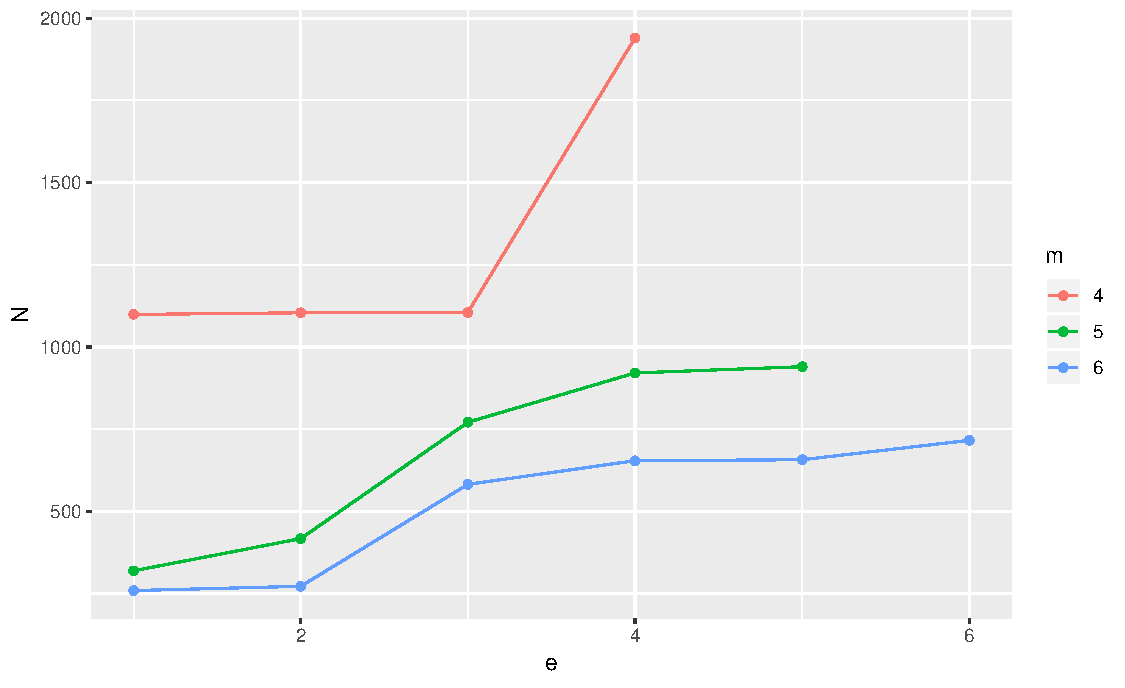
\includegraphics[width=0.8\linewidth, keepaspectratio]{plots/Nvse-m_p6.pdf}
	\caption{Nombre d'itérations $N$ nécessaires pour faire converger $e$ valeurs propres pour différentes tailles de sous-espace de Krylov $m$ et une précision $p=\SI{e-6}{}$ \label{fig:Nvse-m_p6}}
\end{figure}

\begin{figure}
	\centering
	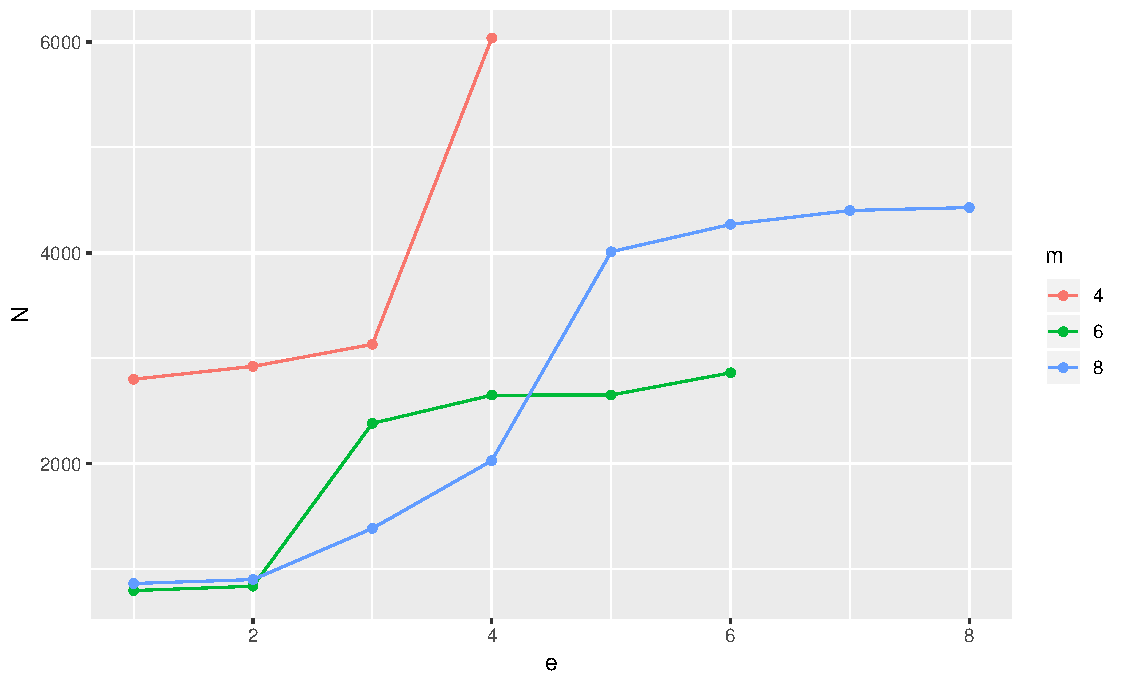
\includegraphics[width=0.8\linewidth, keepaspectratio]{plots/Nvse-m_p8.pdf}
	\caption{Nombre d'itérations $N$ nécessaires pour faire converger $e$ valeurs propres pour différentes tailles de sous-espace de Krylov $m$ et une précision $p=\SI{e-8}{}$ \label{fig:Nvse-m_p8}}
\end{figure}

\begin{figure}
	\centering
	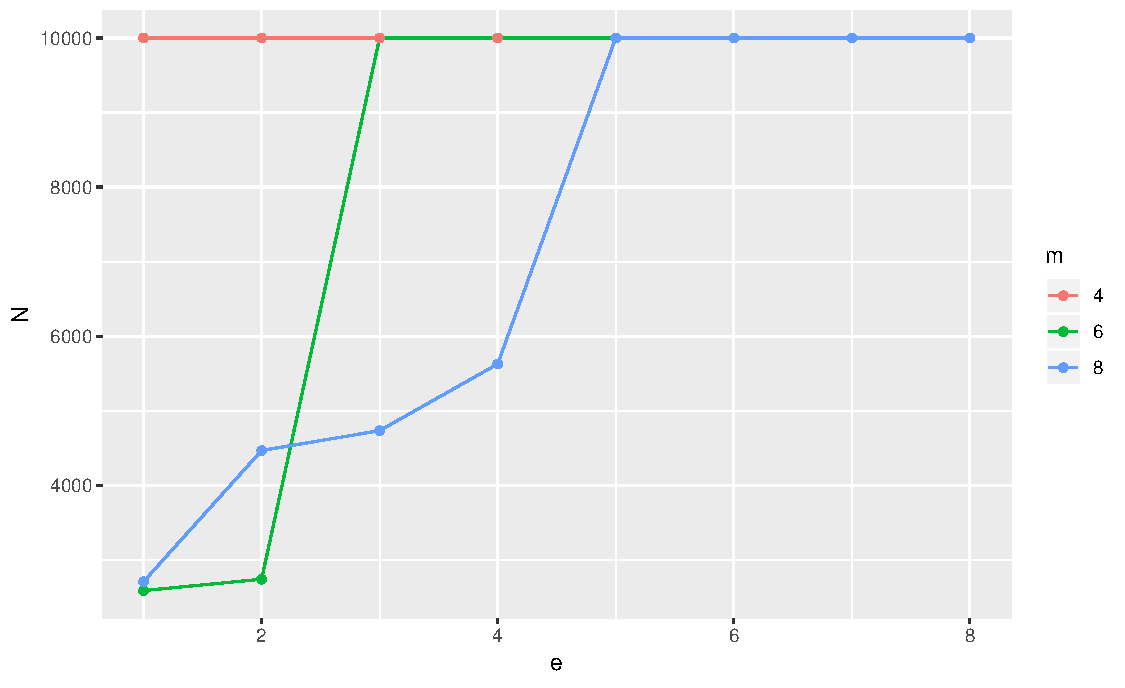
\includegraphics[width=0.8\linewidth, keepaspectratio]{plots/Nvse-m_p10.pdf}
	\caption{Nombre d'itérations $N$ nécessaires pour faire converger $e$ valeurs propres pour différentes tailles de sous-espace de Krylov $m$ et une précision $p=\SI{e-10}{}$ \label{fig:Nvse-m_p10}}
\end{figure}

\begin{figure}
	\centering
	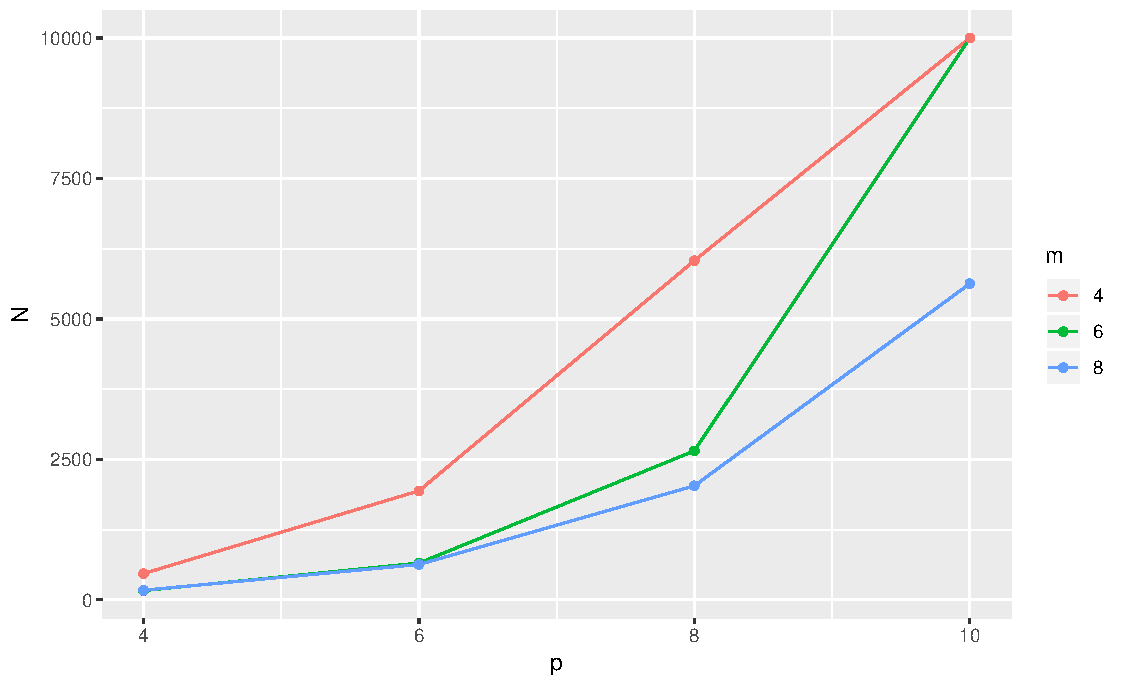
\includegraphics[width=0.8\linewidth, keepaspectratio]{plots/Nvsp-m_e4.pdf}
	\caption{Nombre d'itérations $N$ nécessaires pour faire converger $e = 4$ valeurs propres pour différentes tailles de sous-espace de Krylov $m$ et une précision $p$ \label{fig:Nvsp-m_e4}}
\end{figure}


% \bibliographystyle{unsrt}
% \bibliography{synopsis.bib}

%\input{appendix}

\end{document}
